\section{Linear Programming Optimization}

Linear programming is a commonly used techniques in optimization. In linear programming, we want to optimize (maximize or minimize) a linear function, subject to a set of linear inequalities (called linear constraints). 

\begin{definition}[Linear Constraint] \index{linear function} \index{linear equality} \index{linear inequality} \index{linear constraint}
    Given a set of real numbers $a_1,a_2,\ldots,a_n$ and a set of variables $x_1,x_2,\ldots,x_n$, a \textbf{linear function} $f$ on those variables is
    $$
    f(x_1,\ldots,x_n) = a_1x_1 + a_2x_2 + \cdots + a_nx_n = \sum_{j=1}^n a_jx_j
    $$
    If $b$ is a real number and $f$ is a linear function, then $f(x_1,\ldots,x_n) = b$ is a linear equality ,and $(x_1,\ldots,x_n) \leq b$ and $(x_1,\ldots,x_n) \geq b$ are linear inequalities. Both linear equalities and linear inequalities are called \textbf{linear constraints}.
\end{definition}

Geometrically, a linear function forms a line in $\R^n$. A linear inequality forms a half-space in $\R^n$. All possible solutions to a linear program lies in a convex region called the \textbf{feasible region}. If no such region exsits (no solution satisfies all the contraints), we say the optimization problem is \textbf{infeasible}. The function we wish to optimize is called the \textbf{objective function}, and the value of the objective function evaluated at a particular point is called the \textbf{objective value} at that point. The goal of the linear programming problem is to find a feasible solution that maximizes/minimizes the objective value.

\begin{theorem}[Feasible Region for Linear Programming is Convex]
    Let $\mathbf{x}_1,\mathbf{x}_2 \in \R^n$ be two feasible solutions to the linear programming problem, satisfying some particular constraints. Then, for all $\lambda \in [0,1]$, $\lambda\mathbf{x}_1 + (1-\lambda)\mathbf{x}_2$ is also a solution that satisfies the same constraints.
\end{theorem}

\begin{proof}
    Without loss of generality, suppose that the constraints are given as a system of linear equations $\mathbf{A}\mathbf{x} = \mathbf{b}$. Let $\lambda \in [0,1]$ be arbitrary.
    $$
    \begin{aligned}
        \mathbf{A}(\lambda\mathbf{x}_1 + (1-\lambda)\mathbf{x}_2) &= \lambda\mathbf{A}\mathbf{x}_1 + \mathbf{A}\mathbf{x}_2 - \lambda\mathbf{A}\mathbf{x}_2 \\
        &= \lambda \mathbf{b} + \mathbf{b} - \lambda \mathbf{b} \\
        &= \mathbf{b}
    \end{aligned}
    $$
    Hence, $\lambda\mathbf{x}_1 + (1-\lambda)\mathbf{x}_2$ is also a solution to the system of linear equation and thus is a feasible solution.
\end{proof}

Figure \ref{fig:lp-feasible-region} shows a geometric representation of a linear programming problem with the objective function $x_1+x_2$.

\begin{figure}[htbp]
    \centering
    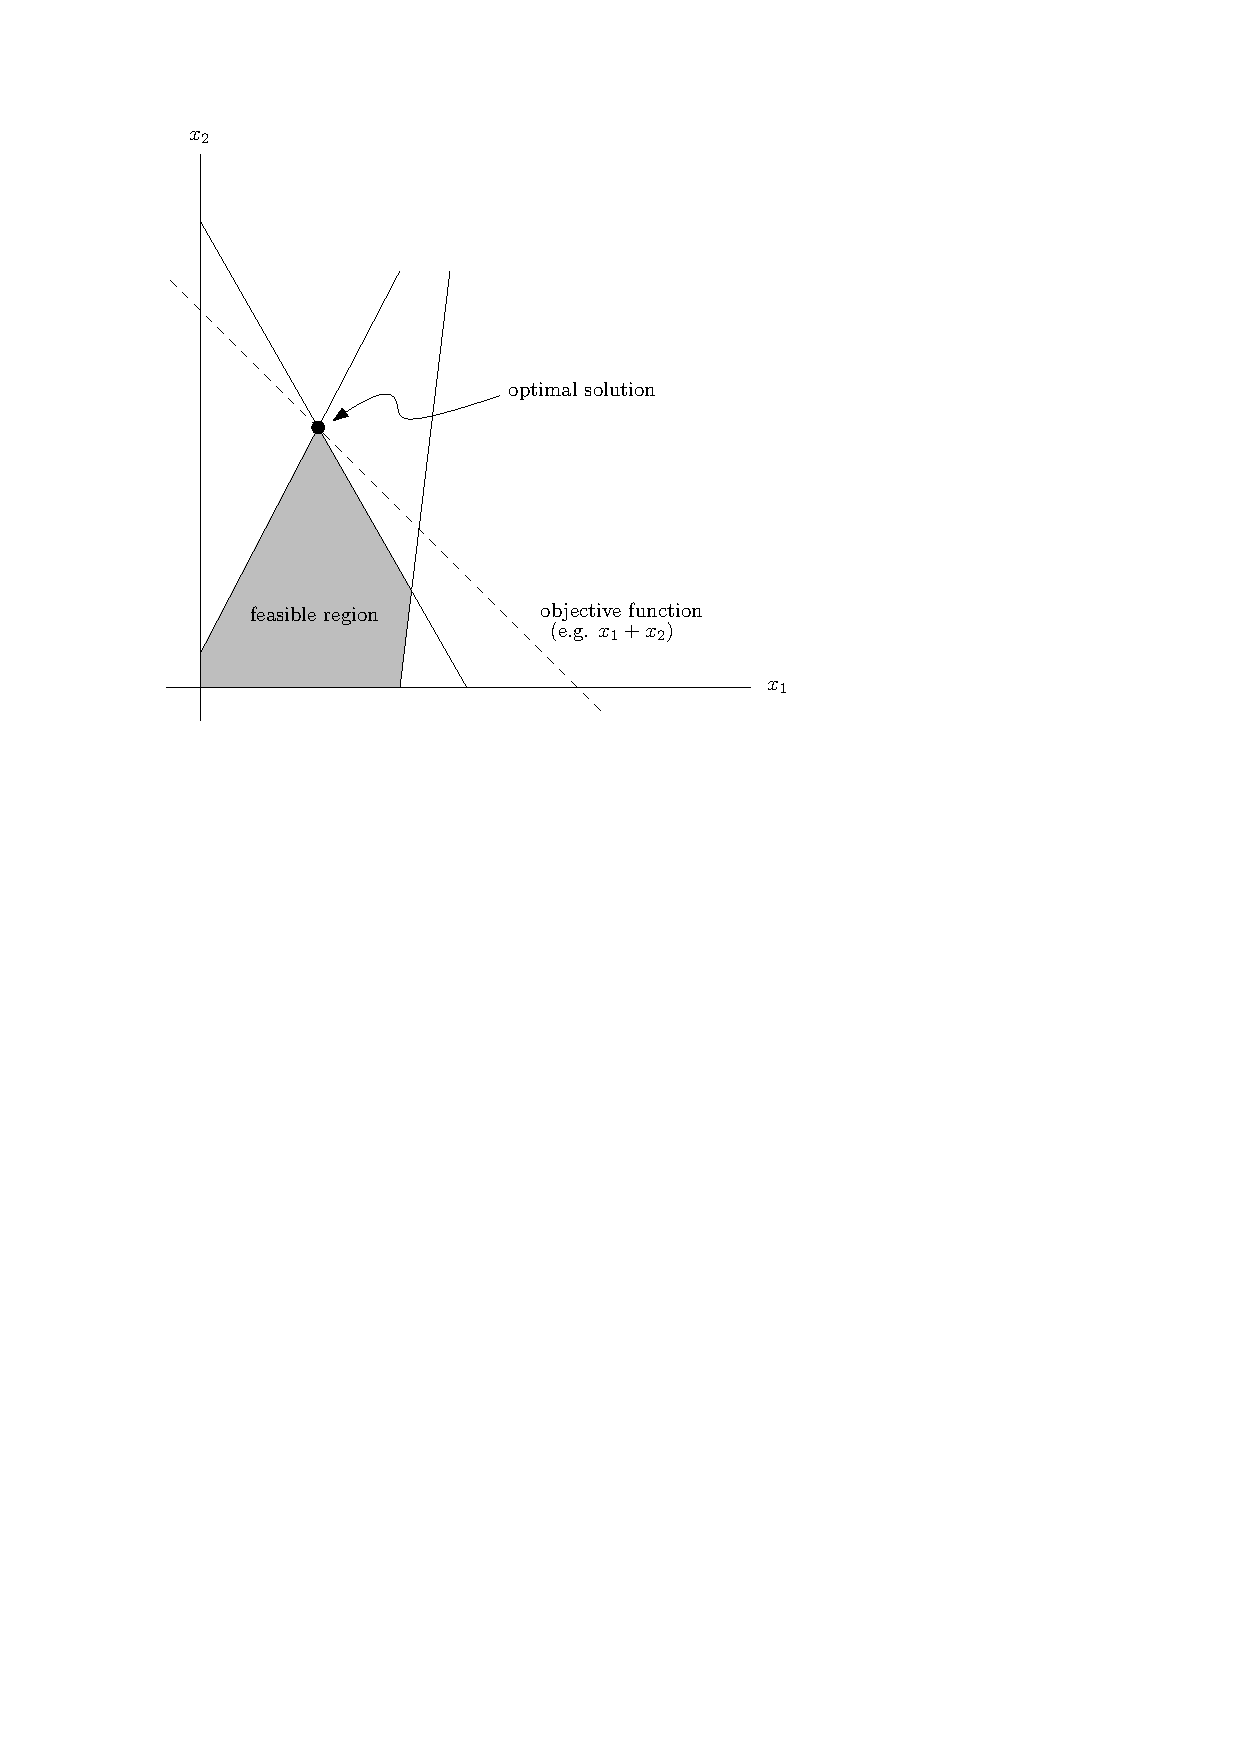
\includegraphics[width=0.6\linewidth]{lp/lp-feasible-region.pdf}
    \caption{A linear programming problem with 2 variables, 4 linear constraints (solid lines), and objective function $x_1+x_2$ (dashed line).}
    \label{fig:lp-feasible-region}
\end{figure}

\section{Standard and Slack Forms}

\subsection{Standard Form}

In standard form, we are given $n$ real numbers $c_1,\ldots,c_n$, $m$ real numbers $b_1,\ldots,b_m$, and $mn$ real numbers $a_{ij}$ for $i \in \{1,\ldots,m\}$ and $j \in \{1,\ldots,n\}$. We wish to

Maximize $\displaystyle \sum_{j=1}^n c_j x_j$ \\
Subject to
\[
    \begin{aligned}
        \sum_{j=1}^n a_{ij} x_j &\leq b_1 & \text{for $i = 1,\ldots,m$} \\
        x_j &\geq 0 & \text{for $j = 1,\ldots,n$}
    \end{aligned}
\]

or, equivalently, in vectorized form

Maximize $\mathbf{c}^\top \mathbf{x}$ \\
Subject to $\mathbf{A}\mathbf{x} \leq \mathbf{b}$ and $\mathbf{x} \geq \boldsymbol{0}$,

where $\mathbf{c}$ is an $n$-vector, $\mathbf{x}$ is an $n$-vector, $\mathbf{b}$ is an $m$-vector, and $\mathbf{A}$ is an $m \times n$ matrix. This can also be written in as a tuple $(\mathbf{A},\mathbf{b},\mathbf{c})$ as a shorthand.

This vectorized form is often used in machine learning because vectorized operations can be carried out more quickly using the GPU.

\subsection{Conversion From Non-standard Form to Standard Form}

A linear programming problem might not be in standard form, but it is easy to convert from non-standard form to standard form.

If \begin{itemize}
    \item the objective is minimization rather than maximization $\Rightarrow$ flip the sign of coefficients;
    \item there are variables without nonnegativity constraints $\Rightarrow$ say a variable $x_j$ does not have  nonnegativity constraints, replace $x_j$ with $x_j' - x_j''$ and add constraints $x_j' \geq 0$ and $x_j'' \geq 0$;
    \item the constraints are equality constraints rather than $\leq$ $\Rightarrow$ replace the constraint with two non-strict inequality constraints ($\leq$ and $\geq$);
    \item the constraints are in the opposite direction ($\geq$ instead of $\leq$) $\Rightarrow$ multiply both sides by -1 
\end{itemize}

\subsection{Slack Form}

Maximize $\displaystyle z = v + \sum_{j=1}^n c_j x_j$ \\
Subject to
\[
    \begin{aligned}
        s_i &= b_1 - \sum_{j=1}^n a_{ij} x_j & \text{for $i = 1,\ldots,m$} \\
        x_j,s_i &\geq 0 & \text{for $j = 1,\ldots,n$ and $i = 1,\ldots,m$ }
    \end{aligned}
\]

or, equivalently, in vectorized form

Maximize $z = v + \mathbf{c}^\top \mathbf{x}$ \\
Subject to $\mathbf{s} = \mathbf{b} - \mathbf{A}\mathbf{x}$ and $\mathbf{x},\mathbf{s} \geq \boldsymbol{0}$.

We call the variables on the left-hand side of the equality constraints the \textbf{basic variables}, and the ones on the right-hand side the \textbf{non-basic variables}.

Similarly, a slack from can be concisely defined by a tuple $(N,B,\mathbf{A},\mathbf{b},\mathbf{c},v)$, where $N$ is the set of indices of the non-basic variables, $B$ is the set of indices of the basic variables such that $|N| = n$, $|B|=m$ and $N \cup B = \{1,2,\ldots,n+m\}$.

It is called the slack from because the variable $s_i$ (or in vectorized form $\mathbf{s}$) measures remaining ``slack'' or difference between two sides of the original inequality constraints. This is related to the simplex algorithm where we increase the non-basic variables as much as possible until we hit a bottleneck -- having no more slack for that non-basic variable.
